\begin{figure*}[t]
\centering
\ifbilingual
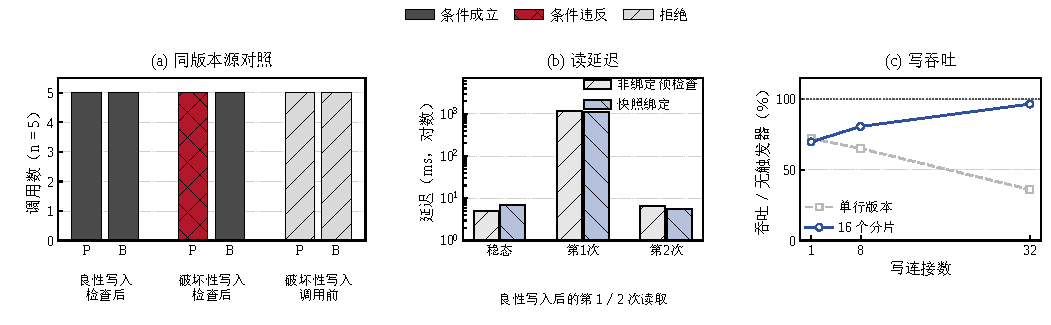
\includegraphics[width=\textwidth]{figures/snapshot-control-zh}
\else
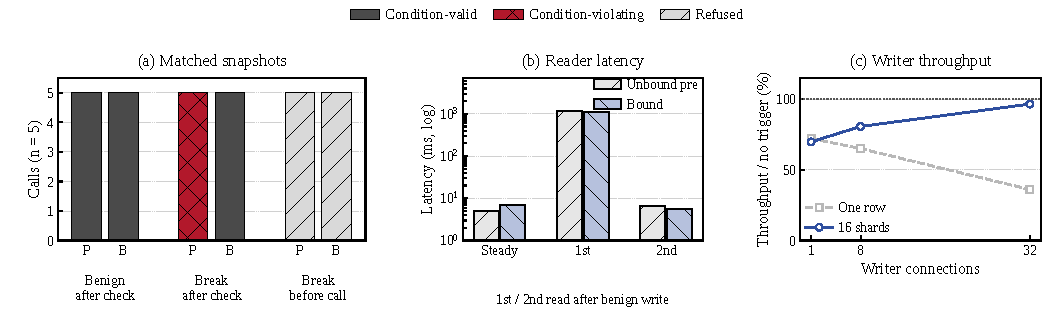
\includegraphics[width=\textwidth]{figures/snapshot-control}
\fi
\caption{\bt{Snapshot validity and overhead. (a) Matched-version control, five calls per mode/schedule: P releases the checked snapshot; B retains it. (b) Read latency: mean of two run medians. (c) Write throughput: median of three runs, normalized to no version trigger.}{快照有效性与开销。(a) 同版本源对照，每种模式／顺序五次调用：P 释放核验快照，B 保留快照。(b) 读延迟：两次运行中位数的均值。(c) 写吞吐：三次运行中位数，相对无版本触发器归一化。}}
\label{fig:snapshot-control}
\Description{Three panels distinguish controlled safety counts from performance measurements. In panel a, both modes return condition-valid results after benign writes. A breaking commit after validation yields five condition-violating precheck results and five valid snapshot-bound results. A breaking commit before invocation makes both modes refuse. Panels b and c show unbound read latency and version-trigger write throughput from separate experiments; artificial barrier waits are never used as performance samples.}
\end{figure*}
